%*****************************************
\chapter{Related Work}\label{ch:Related Work}
%*****************************************
\section{Review of Learning to rank Algorithms}\label{ch:Related Work1}
Learning to rank is a supervised machine learning process. For each given query-document pair, we extract features, and obtain real data annotations through log mining or manual annotation methods. Then through the rank model, the output can be similar to the real ranking list. There are three types of most used learning to rank algorithms : Pointwise, Pairwise and Listwise.
\subsection{Pointwise}
The processing object of Pointwise way is a single document. After converting the document into a feature vector, the learning system scores the document according to the classification or regression function learned from the training data. The score is the search result. Scoring formula is as follows:
\begin{equation}
\begin{aligned}
\mathrm{score} =  \mathbf w \cdot \mathbf x
\end{aligned}
\label{eqn:eq1}
\end{equation}
where  $ w $ is the weight of each dimension of the feature, and $ x $ is the feature vector converted from the doc-query. In the Ranking problem, the label of the training sample we used is not a score, but a label with a strong and weak grading, such as $Perfect> Excellent> Good> Fair> Bad$. In order to map the score to the hierarchical label, 5 thresholds need to be set. If the score falls between two adjacent thresholds, then it is divided into the corresponding label. Most common Pointwise algorithms include: PRank~\cite{crammer2002pranking}, McRank~\cite{Li:2007:MLR:2981562.2981675}, OAP-BPM~\cite{harrington2003online} and 
OPRF~\cite{Fuhr:1989:OPR:65943.65944}. In the following we make a brief introduction to PRank and McRank.

\subsubsection{PRank}
In this algorithm, the dataset can be denoted as: $X_{T\times n}$, $y$, $y\in {1, 2, 3, \dots, k}$, where $X_{T\times n}$ is features of $ T $ training samples , the feature dimension is $ n $, and the training target $ y $ has $k$ number of values.
The goal of PRank is to train a ranking rule $H$: $ R ^ n \rightarrow y$, that is, to project sample features onto $ k $ levels. 
$ H $ is defined as follows: 
\begin{equation}
\begin{aligned}
H(\mathbf x)=\min_{r \in {1, 2, 3, \dots, k}}\{r: \mathbf w \cdot \mathbf x - b_r < 0\}
\end{aligned}
\label{eqn:eq2}
\end{equation}
 Where $ w $ and $b_r, r \in {1, 2, 3, \dots, k}$ are model parameters. $\mathbf w \cdot \mathbf x$ is the score mentioned above, $ k $ number of $b_r$ is the thresholds, and $b_1 \le \dots \le b_ {k-1} \le b_k = \infty$. The main task of the PRank model is to predict these two sets of parameters $ s $ and $b_r$, $r \in {1, 2, 3, \dots, k}$, the method of updating the parameters of PRank is similar to the stochastic gradient descent , the parameters are updated every time when a sample is predicted incorrectly..

\subsubsection{McRank}
McRank is another classic Pointwise algorithm. $DCG$ (Discounted Cumulative Gain) is a indicator for evaluating the quality of a rank in the field of information retrieval. Assuming that a ranking algorithm is used to rank $ n $ documents under a specified query, you can get $DCG$ as follows:
\begin{equation}
\begin{aligned}
DCG=\sum_{i=1}^{n}c_{[\pi_i]}(2^{y_i}-1)
\end{aligned}
\label{eqn:eq3}
\end{equation}
where $ i $ represents the index order of the original document, $ c_ {[\pi_i]} = log (i + 1) $, and $ y_i $ represents the relevance level between the corresponding document and query, it is represented by $ \{0, 1, 2,3,4 \} $, 4 corresponds to a “perfect” relevance and 0 corresponds to a “poor” relevance. The larger the $DCG$ value, the better the ranking. In actual use, it is generally normalized, called $NDCG$ (Normalized discounted cumulative gain). If the $DCG$ value in descending order of gears is the highest, then the ranking problem can be turned into the prediction of document relevance categories specified by the query. That is, multi-classification problem.
For a ranking permutation mapping function $ \pi $, the $DCG$ error is $ DCG_g-DCG _ {\pi} $, where $ DCG_g $ represents the optimal sort, which is sorted in descending order according to the actual query-doc correlation, so there must be:
\begin{equation}
\begin{aligned}
DCG_g \geq DCG _ {\pi} 
\end{aligned}
\label{eqn:eq4}
\end{equation}
Suppose the training data is $\{y_i,x_i\}_i^N$, $y_i$ represents the category, then what will eventually be learned is the probability of each category $p_{i,k}=Pr(y_i=k)$, then the final sort score is:
\begin{equation}
\begin{aligned}
S_i=\sum_{k=0}^{K-1}p_i^kT(k)
\end{aligned}
\label{eqn:eq5}
\end{equation}
where $ T (k) $ represents a function which increases monotonically with the gear, and in McRank $ T (k) =  k $.

Normally the order of ranking is very important, and the Pointwise methods learn the global correlation, but does not penalize the order of the Ranking result. This is the main disadvantage of Pointwise methods.

\subsection{Pairwise}
For a search system, the system returns a list of related documents after receiving a user query, so the key to the problem is to determine the order relationship between documents. The Pointwise methods are calculated entirely from the classification score of a single document, without considering the order relationship between the documents. The Pairwise methods turn the ranking problem into a ranking problem for multiple pairs, comparing the order of different articles.
Classic Pairwise algorithms are: RankNet~\cite{Burges:2005:LRU:1102351.1102363}, RankBoost~\cite{freund2003efficient}, Ranking SVM~\cite{joachims2002optimizing}, GBRank~\cite{zheng2007regression}.
 \subsubsection{RankNet}
Suppose there is now a pair of documents $ D_i $ and $ D_j $, given a target probability $\bar{P}_{i,j}$, to indicate that document $ D_i $ will be ranked before document $ D_j $. We now express the predicted probability of $P(D_i \triangleright D_j)$ in the order of $P_{i,j}$, and define $o_i = f(x_i)$ and $o_{i,j}=f(x_i)-f(x_j)$, then we can use logistic function to represent $ P_ {i, j} $:
\begin{equation}
\begin{aligned}
P_{i,j} = \frac{e^{o_{i,j}}}{1+e^{o_{i,j}}} = \frac{1}{1+e^{-o_{i,j}}}
\end{aligned}
\label{eqn:eq6}
\end{equation}
Where $ o_{i,j} $ is the parameter to be learned. If $ D_i $  is more relevant than $ D_j $, then $P_{i,j}>0.5$, otherwise $P_{i,j}<0.5$. So the sigmoid function is used to make the probability maps to a real number on $[0, 1]$. In order to measure how close the predicted probability $P_{i,j}$ is to the target probability $\bar{P}_{i,j}$, it uses cross entropy as the loss function:
\begin{equation}
\begin{aligned}
C_{i,j} = -\bar{P}_{i,j} log P_{i,j} - (1-\bar{P}_{i,j}) log (1-P_{i,j})
\end{aligned}
\label{eqn:eq7}
\end{equation}
RankNet uses Stochastic Gradient Descent (SGD) to optimize parameters.
However, in many cases, it is not enough to evaluate the ranking based on the number of wrong pairs. Evaluation indexes in information retrieval such as $NDCG$ or $ERR$ only focus on the ranking of the top $k$ results. Because these indexes are not differentiable, RankNet cannot use them as the optimization target to iterate, so there is a gap between RankNet's optimization target and evaluation index of information retrieval.
\subsubsection{RankBoost}
RankBoost's idea is relatively simple, and it is the general idea of binary learning to rank: by constructing the target classifier, the objects in the pair have a relative size relationship. Grouping objects into pairs, such as a set of $r1> r2> r3> r4$, we can form pairs: $(r1, r2), (r1, r3), (r1, r4), (r2, r3), (r3, r4)$, if a pair is positive, then set the label to 1. The remaining pairs, such as $(r2, r1)$, should be set to -1 or 0.
The loss function is the same as defined by AdaBoost and is still defined as an exponential loss, but it is a Pairwise version:
\begin{equation}
\begin{aligned}
L(f;x_{u},x_{v},y_{u,v})=exp(-y_{u,v}(f(x_{u})-f(x_{v})))
\end{aligned}
\label{eqn:eq8}
\end{equation}
\subsubsection{Ranking SVM}
Ranking SVM is another Pairwise ranking algorithm. Given a query $q$, document $d1> d2> d3$, document $d1$ is more relevant than document $d2$, document $d2$ is more relevant than document $d3$. $x1, x2, x3$ are the characteristics of $d1, d2, d3$, respectively. In order to use machine learning for ranking, we turn the ranking problem into a classification problem. Ranking SVM defines new training samples, let $x1-x2, x1-x3, x2-x3$ be positive samples, and $x2-x1, x3-x1, x3-x2$ be negative samples, then train a binary classifier to classify these new training samples.
Ranking SVM aims to minimize the ranking loss while having a large margin, where the ranking learning step can be formulated as follows:
\begin{equation}
\begin{aligned}
& \min \limits_\mathbf{W} \ \frac{1}{2} \sum_{j=1}^{l} \| \mathbf{w}^j \|^2 + \lambda \sum_{i=1}^{n} \frac{1}{|Y_i^+||Y_i^-|} \sum_{p \in Y_i^+} \sum_{q \in Y_i^-} \xi_{pq}^i \\
		& s.t. \ \langle \mathbf{w}^p, \mathbf{x}_i \rangle - \langle \mathbf{w}^q, \mathbf{x}_i \rangle \geq 1 - \xi_{pq}^i, \ (p, q) \in Y_i^{+}  \times Y_i^{-} \\
		& \qquad \xi_{pq}^i \geq 0, \ i = 1,...,n \\ 
\end{aligned}
\label{eqn:eq9}
\end{equation}
where $Y_i^{+}$ (or $Y_i^{-}$) denotes the index set of relevant (or irrelevant) labels associated with the instance $\mathbf{x}_i$, $| \cdot |$ denotes the cardinality of a set, $\xi_{pq}^i$ is the slack variable and $\lambda$ is a tradeoff hyper-parameter which controls the model complexity. Note that it will additionally regularize the bias term $b_j$ when absorbing $b_j$ into $\mathbf{w}^j$, which is different from the original optimization problem that doesn't regularize $b_j$. Ranking SVM has good generalization ability and inherits the advantages of SVM.

But the Pairwise methods also have the following problems: 
The Pairwise method takes into account the relative order of two document pairs, but does not consider the position of the document in the list. The document ranked before the search results is more important. If the front document has a wrong judgment, the cost is significantly higher than the documents that lay behind.
At the same time, the number of related documents varies greatly from different queries, so after conversing to document pairs, some query pairs can have hundreds of corresponding document pairs, while some queries have only a dozen corresponding document pairs. So it is difficult to evaluate the effect.

\subsection{Listwise}
The Listwise methods directly consider the overall sequence and optimize the evaluation index of ranking. The most used Listwise methods are: Adarank~\cite{xu2007adarank}, SoftRank~\cite{taylor2008softrank}, LambdaRank~\cite{burges2007learning}, and LambdaMART~\cite{burges2010ranknet}.

\subsubsection{LambdaRank}
In view of the shortcoming of RankNet, LambdaRank bypasses the loss function and directly defines the gradient. First we look at the gradient of RankNet:
\begin{equation}
\begin{aligned}
\frac{\partial L}{\partial w_k} =
    \sum_{(i, j) \in P}\frac{\partial L_{ij}}{\partial w_k} =
    \sum_{(i, j) \in P}
        \frac{\partial L_{ij}}{\partial s_i}\frac{\partial s_i}{\partial w_k}
            +
        \frac{\partial L_{ij}}{\partial s_j}\frac{\partial s_j}{\partial w_k},
\end{aligned}
\label{eqn:eq10}
\end{equation}
Note the following symmetry:
\begin{equation}
\begin{aligned}
\frac{\partial L_{ij}}{\partial s_i} & {} = \frac{\partial \biggl\{\frac12 (1 - S_{ij})\sigma\cdot(s_i - s_j) + \log\Bigl\{1 + \exp\bigl(-\sigma\cdot(s_i - s_j)\bigr)\Bigr\}\biggr\}}{\partial s_i}\\
 & {}= \frac12 (1 - S_{ij})\sigma - \frac{\sigma}{1 + \exp\bigl(\sigma\cdot(s_i - s_j)\bigr)} \\
 & {}= \sigma\Biggl[\frac12(1 - S_{ij}) - \frac{1}{1 + \exp\bigl(\sigma\cdot(s_i - s_j)\bigr)}\Biggr] \\
 & {}= -\frac{\partial L_{ij}}{\partial s_j}
\end{aligned}
\label{eqn:eq11}
\end{equation}
So define:
\begin{equation}
\begin{aligned}
\lambda_{ij}\mathrel{\stackrel{\mbox{def}}{=}} \frac{\partial L_{ij}}{\partial s_i} = -\frac{\partial L_{ij}}{\partial s_j}
\end{aligned}
\label{eqn:eq12}
\end{equation}
Based on this, the gradient in LambdaRank is:
\begin{equation}
\begin{aligned}
\lambda_{ij}\mathrel{\stackrel{\mbox{def}}{=}} - \frac{\sigma}{1 + \exp\bigl(\sigma\cdot(s_i - s_j)\bigr)}\cdot\lvert\Delta Z_{ij}\rvert
\end{aligned}
\label{eqn:eq13}
\end{equation}
where  $\Delta Z$ indicates that the difference of the evaluation index (the other document orders are unchanged) obtained after exchanging the positions of the documents $D_i$ and $D_j$, from the new calculation, $\lambda_i$ is:
\begin{equation}
\begin{aligned}
\lambda_i = \sum_{j:\{i,j\} \in I} \lambda_{i,j} - \sum_{j:\{j,i\} \in I} \lambda_{i,j}
\end{aligned}
\label{eqn:eq14}
\end{equation}
This gradient represents the direction and intensity of the next iterative optimization. Due to the introduction of the IR evaluation index, Lambda gradient is more concerned about the improvement of the ranking position of high-quality documents that are positioned higher. This effectively avoids the situation of lowering the position of the high-quality document in front. The advantage of LambdaRank over RankNet is that the training speed becomes faster after factoring, and at the same time, evaluation indicators are considered.

\subsubsection{LambdaMART}
LambdaRank redefines the gradient and gives them new physical meaning. Therefore, all models that can be solved using the gradient descent can use this gradient. MART(Multiple Additive Regression Tree) is one of them. MART is an ensemble learning algorithm. Unlike the classic ensemble learning algorithm Adaboost, which uses the errors of the previous round of learners to update the sample weights of the next round of learning, MART fits the residuals generated by the previous round of classifiers each time.

Combining the gradient Lambda and MART is the famous LambdaMART algorithm. The principle of MART is to solve the function directly in the function space. The model's result consists of many trees. The fitting goal of each tree is the gradient of the loss function, in LambdaMART, it is Lambda. LambdaMART's framework is actually MART. The main innovation is that the gradients used in the intermediate calculation are Lambda and Pairwise. The parameters that MART needs to set include: the number of trees $M$, the number of leaf nodes $L$, and the learning rate $v$. These three parameters can be adjusted by the verification set to obtain the optimal parameters. 

LambdaMART has many advantages, it is more suitable for Ranking: instead of traditionally solving the ranking problem by classification or regression, but directly do ranking, and because of the tree model, you can learn different feature combinations.

\subsubsection{ListNet}
In the search scenario, all the query requests are expressed as:

$\begin{matrix} Q= \left ( q^{(1)},q^{(2)},...,q^{(m)} \right ) \end{matrix}$, for each query, there will be a search result. The results are ordered documents. For a query, the search results can be expressed as: $d^{(i)}=\left ( d_1^{(i)}, d_2^{(i)},...,d_{n^i}^{(i)}\right)$. Correspondingly, there will be a score vector representing the score of each search result: $y^{(i)}=\left ( y1^{(i)},y_2^{(i)},...,y_{n^i}^{(i)}\right )$. 
\\
Let $\pi$ represents a certain permutation, $\phi(\cdot )$ is a monotonically increasing function with a positive range. For a certain permutation and its score, the probability of defining the current permutation is:
\begin{equation}
\begin{aligned}
P_s(\pi)=\prod_j^n \frac{\phi(s_{\pi(j)})}{\sum_{k=j}^n \phi(s_{\pi(k)})}
\end{aligned}
\label{eqn:eq15}
\end{equation}
where $s_{\pi(j)}$ is the score of object at position $j$ of permutation $\pi$. The top one probability of object $j$
is defined as:
\begin{equation}
\begin{aligned}
P_s(j) = \frac{\phi(s_j)}{\sum_{k=1}^n \phi(s_k)}
\end{aligned}
\label{eqn:eq16}
\end{equation}
The cross entropy loss function:
\begin{equation}
\begin{aligned}
L(y^{(i)}, z^{(i)}) = - \sum_{j=1}^{n^{(i)}} P_{y^{(i)}}(j) \log P_{z^{(i)}}(j) = - \sum_{j=1}^{n^{(i)}} \frac{\phi(y_j^{(i)})}{\sum_{k=1}^n \phi(y_k^{(i)})} \log \frac{\phi(z_j^{(i)})}{\sum_{k=1}^n \phi(z_k^{(i)})}\end{aligned}
\label{eqn:eq16}
\end{equation}
where $y$ is the actual label and $z$ is the prediction.
ListNet's model is a neural network, it has proven to be a better method than Pairwise. Of course, the complexity of fitting its parameters is also much higher than others.

\newpage
\section{Review of Model Interpretability}
Machine learning business applications target output decision making. Interpretability refers to the degree to which humans can understand the reason for a decision. The more interpretable a machine learning model is, the easier it is for people to understand why certain decisions or predictions are made. Model interpretability refers to the understanding of the internal mechanism of the model and the results of the model. It‘s importance is reflected in: the modeling phase, assisting developers to understand the model, comparing and selecting models, and optimizing models. In the operational phase, explaining the internal mechanism of the model to the business party and explaining the model results. For example, a fund recommendation model needs to explain: why a certain fund is recommended for this user or not.

\paragraph{Model Improvement}
Understanding the characteristics of indicators, classification, and predictions, and then why a machine learning model makes such a decision, and which features play the most important role in the decision, allows us to judge whether the model is consistent with common sense. Knowing how the model uses features to make predictions, we can intuitively determine whether our model captures meaningful features and whether the model can be generalized to the predictions of other samples.

\paragraph{Model Credibility and Transparency}
Understanding machine learning models is necessary to improve the credibility of the model and to provide transparency in reviewing and predicting the results. It is unrealistic for black box models to determine people's lives, such as loans and prison criminal law. Another area that questions the credibility of machine learning results is medicine, and model results directly determine the life and death of patients. Machine learning models are very accurate in distinguishing malignant tumors from different types of benign tumors, but we still need experts to explain the diagnosis and explain why a machine learning model will classify a patient's tumor as benign or malignant and help doctors trust and use machine learning models to support their work.
\paragraph{Prevent Biases}
Biased models are often caused by biased samples. If the data contains subtle biases, the model learns and thinks the fit is good. A well-known example is the use of machine learning models to suggest convictions and sentencing for prisoners, which clearly reflects the inherent bias of the justice system over racial inequality. Other examples include machine learning models for recruitment that reveal gender bias in specific positions, such as male software engineers and female nurses.

~\\
The explaination attempts to understand and explain these decisions made by the response function, namely, what, why, and how. The key to model interpretation is transparency, the ability to question, and the ease with which humans understand model decisions. The three most important aspects of model interpretation are explained below:
\paragraph{What drives the model's predictions?}
 We should be able to query our model and identify potential feature interactions to understand which features may be important in the model's decision strategy. This ensures the fairness of the model.
\paragraph{Why does the model make a decision?}
We should also be able to verify and justify why certain key features are responsible for driving certain decisions made by the model during the forecast period. This ensures the reliability of the model.
\paragraph{How do we trust model predictions?}
We should be able to evaluate and validate any data point and how the model makes decisions about it. This should be provable and easy to understand for the key stakeholders where the model works as expected. This ensures the transparency of the model.

\subsection{Interpretable Model}
Among the algorithms for machine learning, some models are difficult to interpret, such as deep neural networks. Deep neural networks can fit highly complex data with huge parameters, but how to interpret these is very difficult. However, there are still quite a few algorithms that can be easily explained.

For example, linear regression. Linear regression is easy to use and can also guarantee to find the optimal solution. But not all problems are linear after all. Another example of an interpretable model is decision tree. The decision tree clearly gives the basis for prediction. To explain how a decision tree predicts is very simple, it starts from the root node, starts branching according to all features, and reaches the leaf node to find the final prediction.

Decision trees can well capture the interactions and dependencies between features. The tree structure can also be well visualized. However, the decision tree is difficult to handle the linear relationship. It is not smooth and unstable, and a small change in feature data may change the construction of the entire tree. As the nodes and levels of the tree become larger, it becomes more difficult to explain the entire decision-making process. There are much other interpretable models, such as logistic regression, general linear models, Naive Bayes, Kmeans, etc.


\subsection{Model-agnostic Methods}
After all, the types of interpretable models are limited, and we hope to find some ways to provide explanations for any black box machine learning model. Here we need a model-agnostic methods.
\subsubsection{Partial Dependence Plot (PDP)}
PDP is used to represent the impact of one or two features in a model on the prediction. The PDP chart below shows three characteristics of temperature, humidity, and wind speed on the number of cyclists. Each graph is a trend assuming that other features are constant.

\begin{figure}[H]
\centering
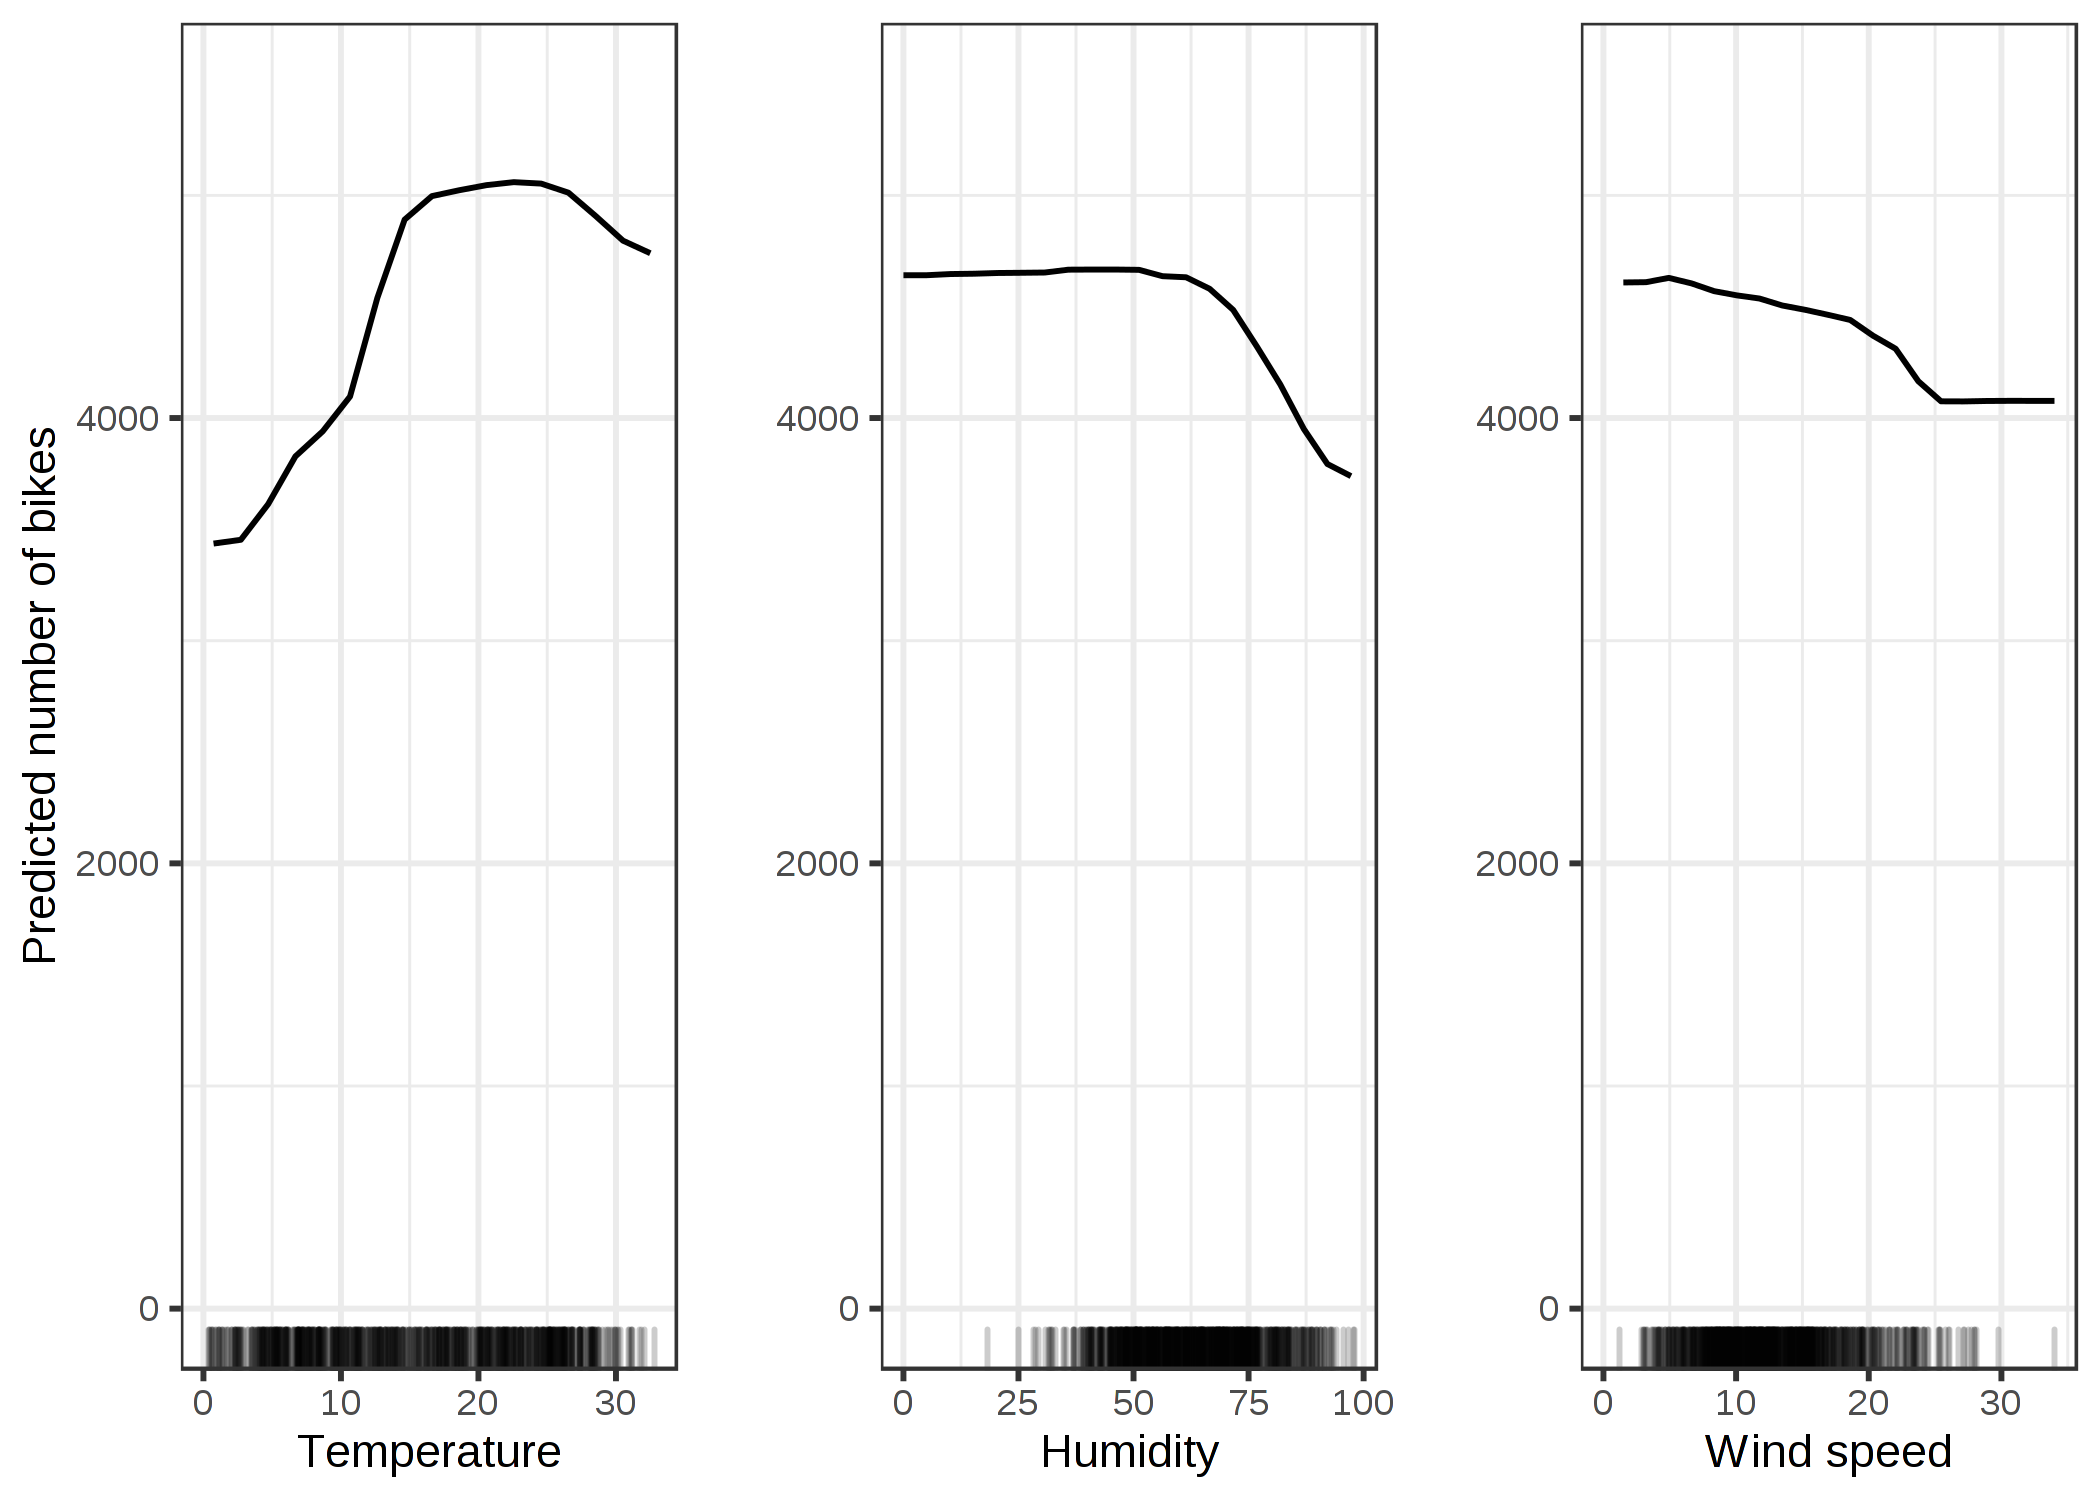
\includegraphics[width=0.6\columnwidth]{gfx/pdp-bike-1.png}
\caption{PDPs for the bicycle count prediction model and temperature, humidity and wind speed.~\cite{molnar2019}}
\label{fig:pdp-bike}
\end{figure}

PDP diagrams are very intuitive and easy to calculate and generate. However, PDP maps can only reflect two features at most, because more than three-dimensional maps cannot be represented by current technology. At the same time, the independence assumption is the biggest problem of PDP.

\subsubsection{Individual Conditional Expectation (ICE)}
The ICE and PDP charts reflect a consistent trend, but include all samples. Similar to PDP, ICE's independence assumption and inability to characterize more than two features are it's limitations. At the same time, as the number of samples increases, the graph will become quite crowded.
\begin{figure}[H]
\centering
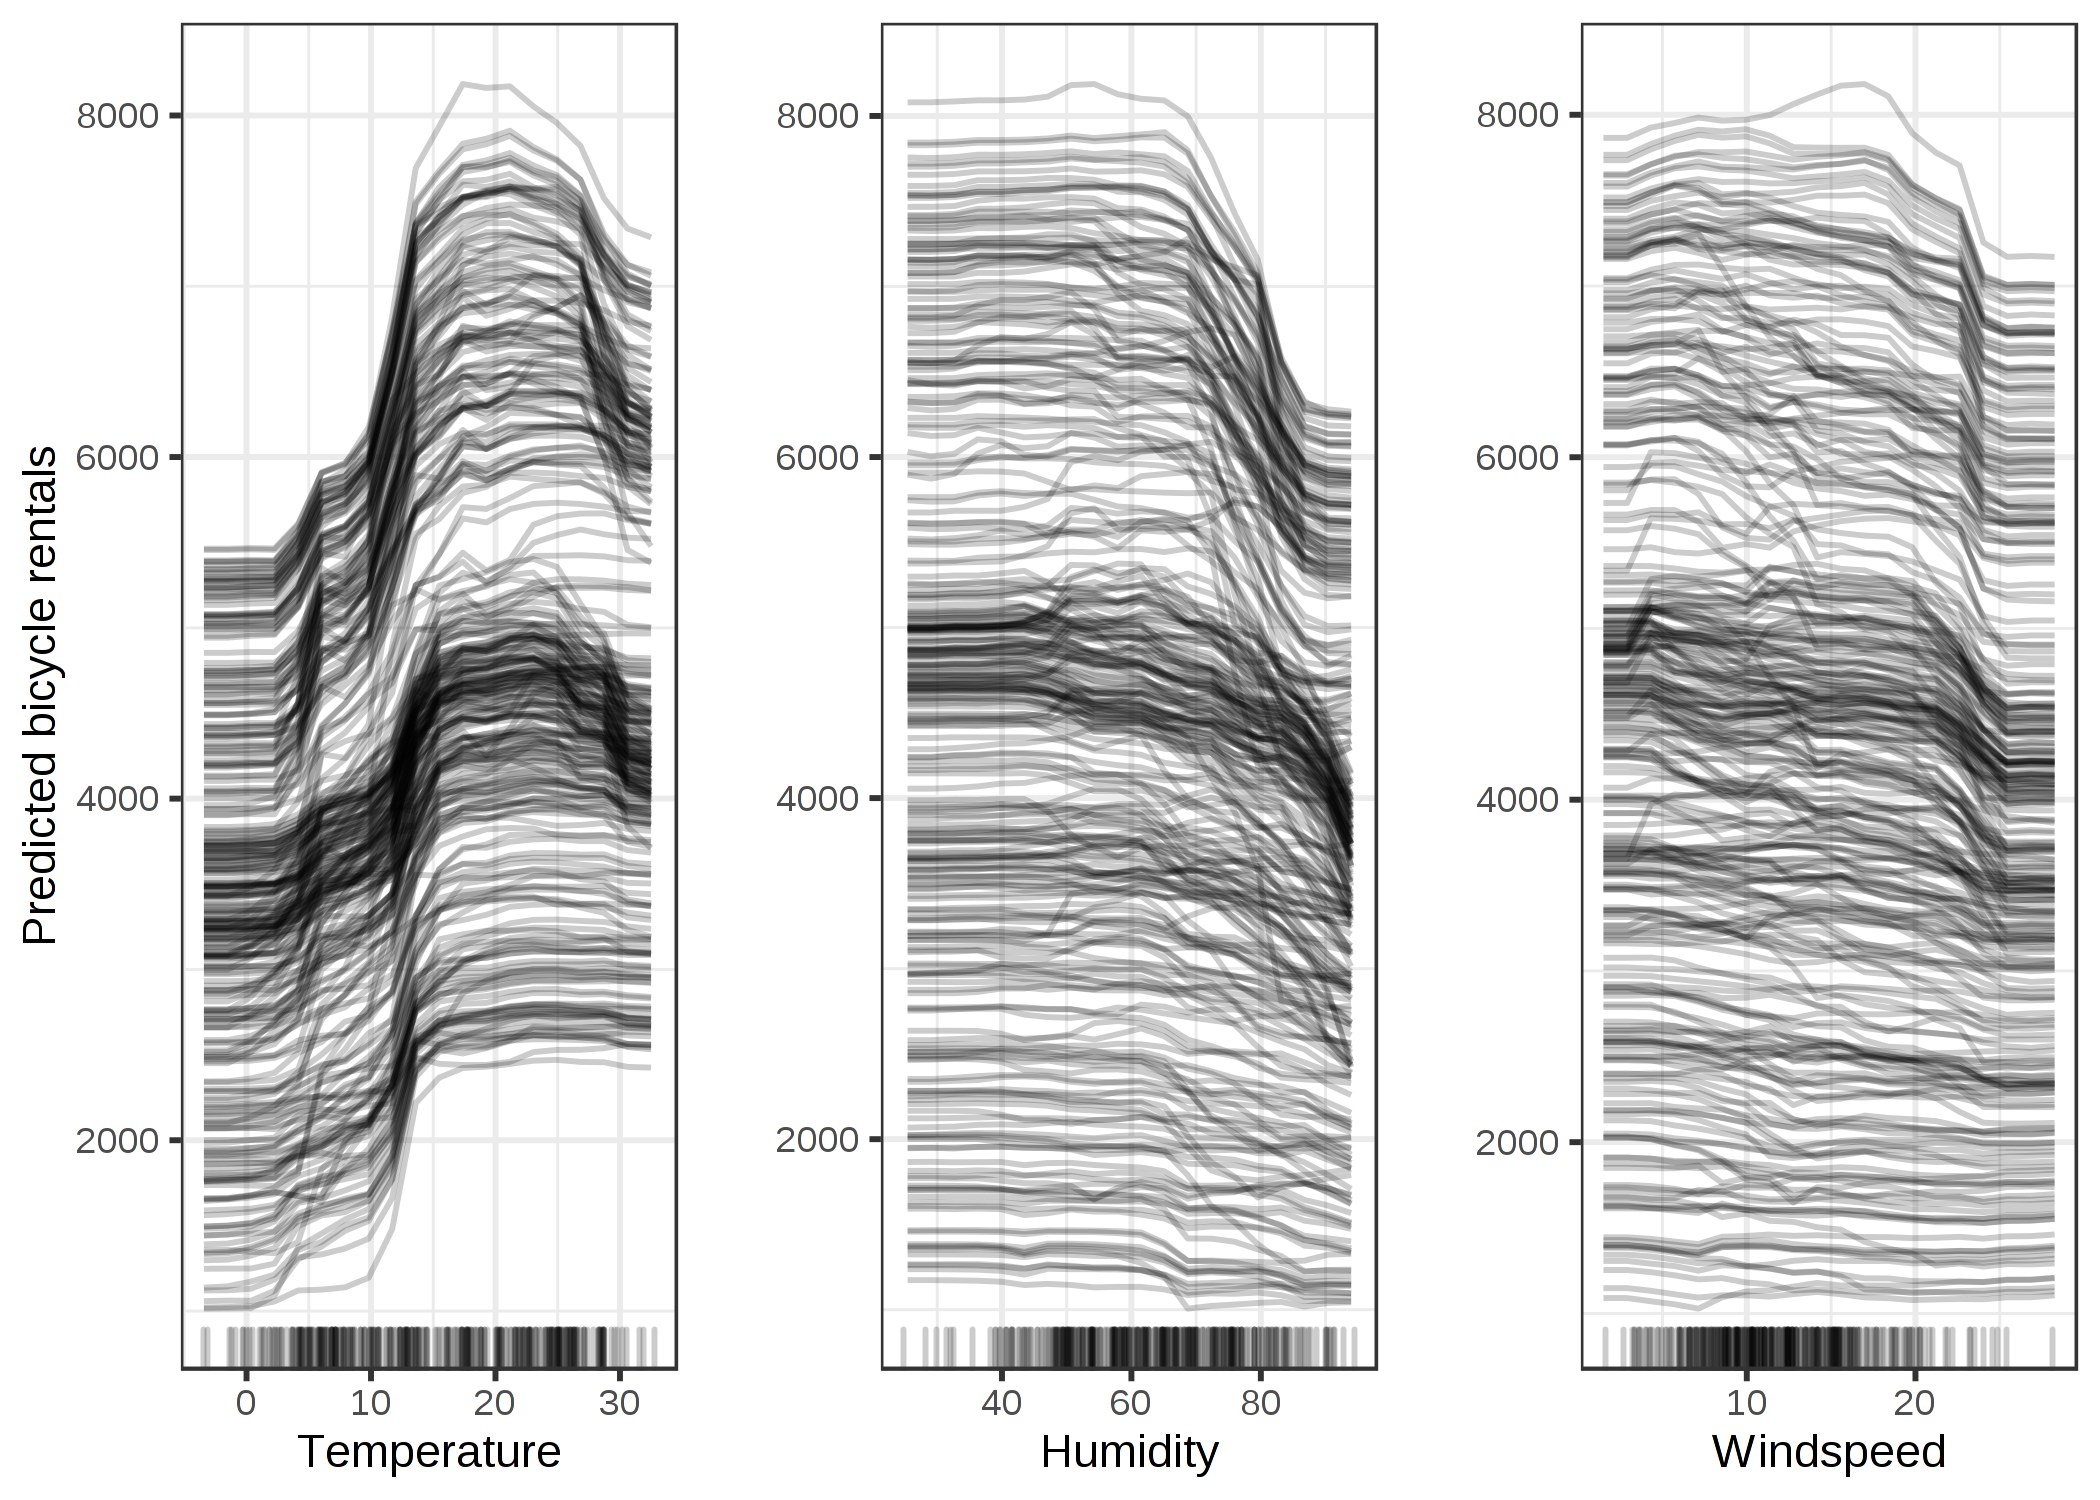
\includegraphics[width=0.6\columnwidth]{gfx/ice-bike-1.png}
\caption{ ICE plots of predicted bicycle rentals by weather conditions.~\cite{molnar2019}}
\label{fig:ice-bike}
\end{figure}

\subsubsection{Feature Interaction}
For example, a model has two features, then the model can be a constant and a term containing only the first feature and a term containing only the second feature and an interaction term between the two features. 
\begin{figure}[H]
\centering
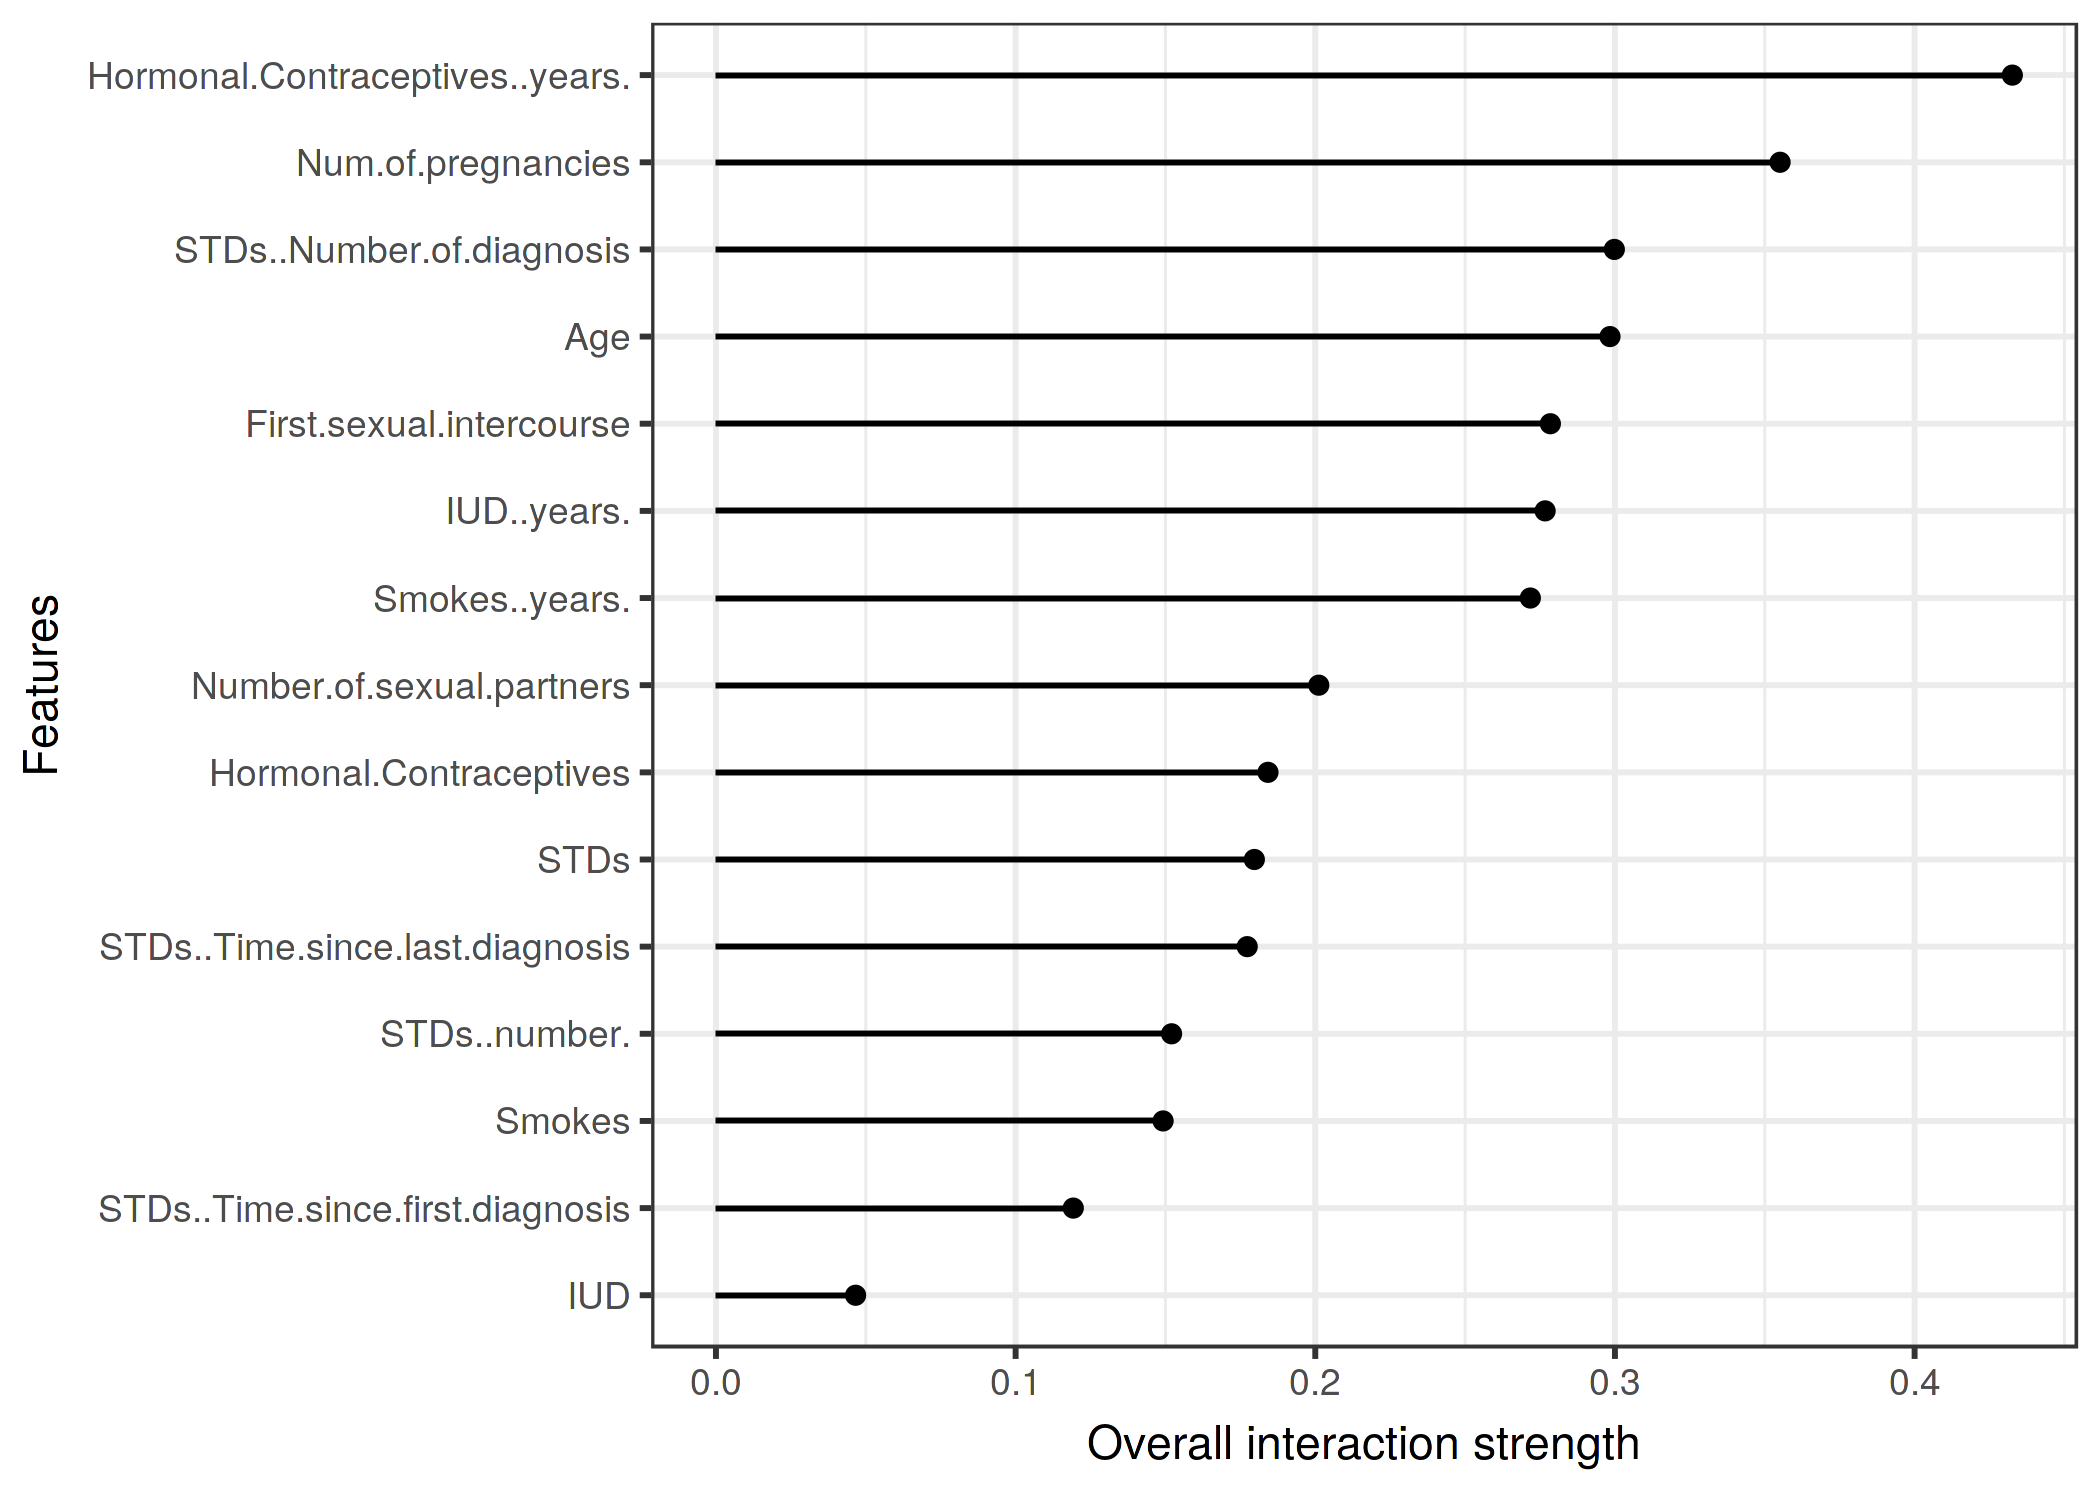
\includegraphics[width=0.6\columnwidth]{gfx/interaction-cervical-1.png}
\caption{The interaction strength (H-statistic) for each feature with all other features for a support vector machine predicting bicycle rentals.~\cite{molnar2019}}
\label{fig:interaction}
\end{figure}
~\\Using Friedman's H-statistic theory, we can calculate feature interactions. H-statistic calculations are resource-intensive and the results are not very stable.

\subsubsection{Feature Importance}
The definition of feature importance is the change caused by the prediction error when the value of a feature is changed. When we change a feature, the prediction error changes greatly, indicating that the feature has a great influence. On the contrary, if the value of another feature is changed, it has no effect on the error of the prediction result. It doesn't matter.
\begin{figure}[H]
\centering
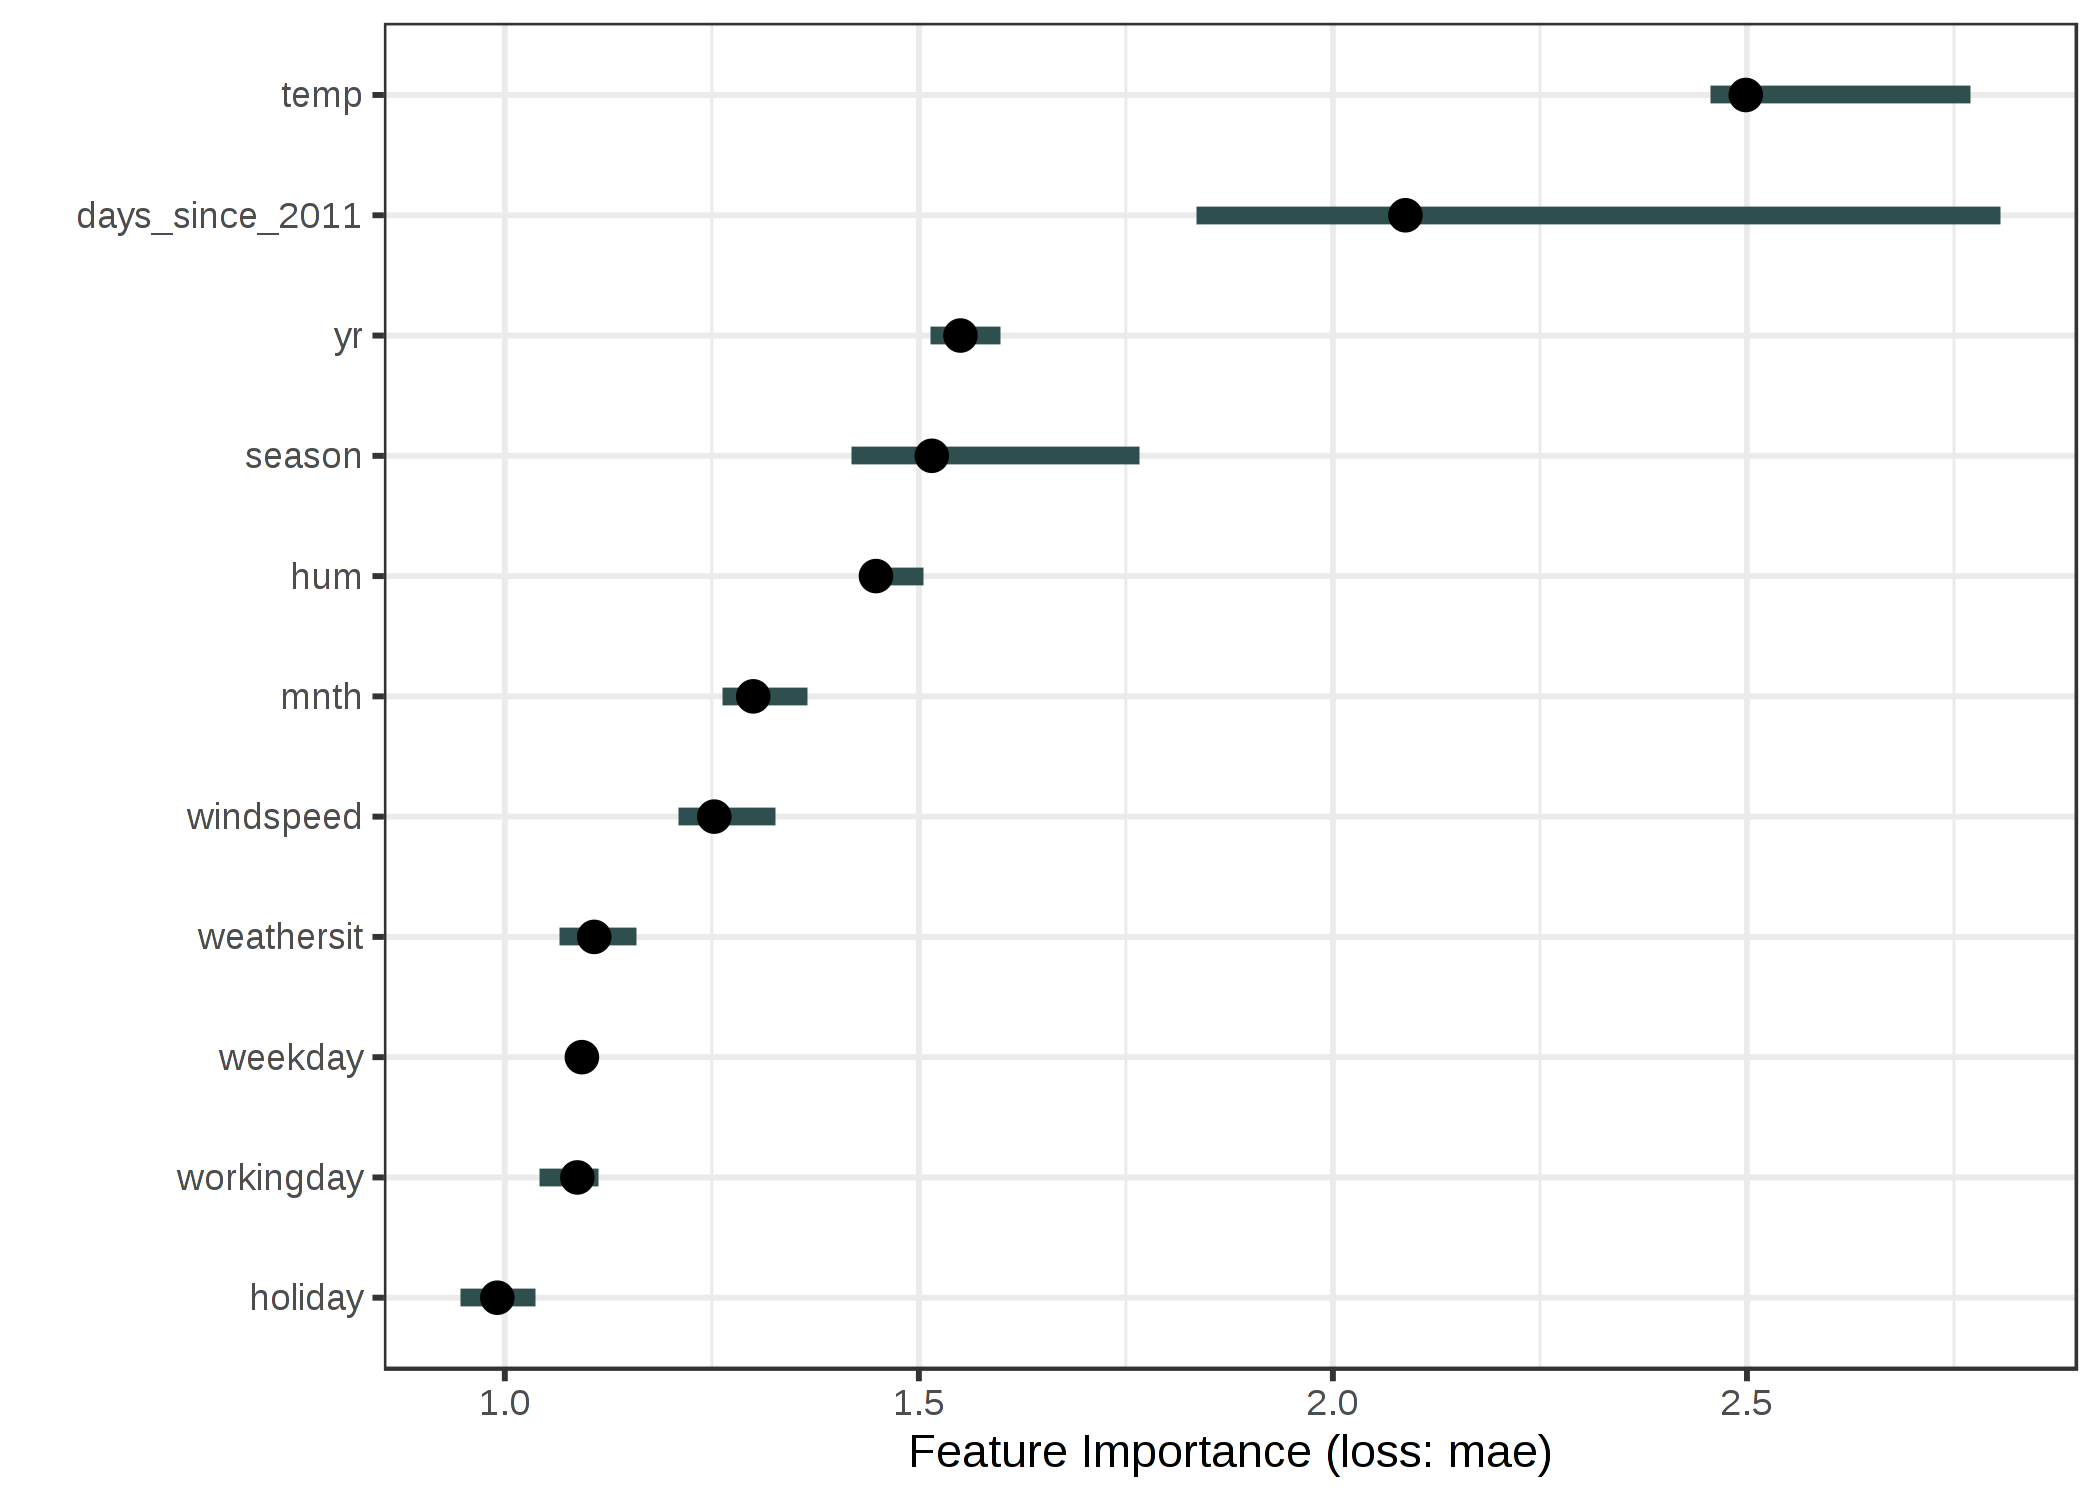
\includegraphics[width=0.6\columnwidth]{gfx/importance-bike-1.png}
\caption{The importance for each of the features in predicting bike counts with a support vector machine.~\cite{molnar2019}}
\label{fig:importance}
\end{figure}

\subsubsection{Surrogate Model}
The substitute model is a simpler model that can be interpreted. For the input and prediction of the black box model, a substitute is trained. This model is used to explain the complex black box model.
The training processes of the alternative model are as follows:
\\\\1. Choose a data set X (can be the same or different from the training set)
\\\\2. Predicting Y with a trained black box model.
\\\\3. Choose an interpretable model, such as a linear regression or decision tree.
\\\\4. Train this interpretable model with the previous dataset X and prediction Y.
Verify the differences between explainable models and black box models. Alternative models are flexible, intuitive and easy to implement,but it is an interpretation of the black box model, not an interpretation of the data.

\subsubsection{LIME}
What is LIME? Which is a local interprentable model-agnostic explanation proposed by Ribeiro in 2016~\cite{ribeiro2016i}. They use $G$ to represent models that may be used for interpretation, it can be a linear model, a tree model or a simple set of rules, use $g \in G$ to represent a specific interpretive model, that is, $g$ is a model trained on $x^{\prime} \in \lbrace 0,1 \rbrace ^{d^\prime}$. For the interpretability of the model, the model cannot be too complicated. Therefore, we use $\Omega(g)$ to represent the complexity of the model. We need to limit the complexity of the model to a certain range. In addition, the $g$ that we use to explain the model should be as close to $f$ as possible, at least to maintain the authenticity around the sample $x$ that needs to be explained. The way we use to define the surrounding is $\pi_x(z)$, in fact, it indicates how far away $z$ is from the sample $x$, the closer, the greater the weight should be. So the explaination of the model is:
\begin{equation}
\begin{aligned}
\xi(x) = \mathop {argmin}_{g\in G} L(f, g, \pi_x) + \Omega(g)
\end{aligned}
\label{eqn:eq1}
\end{equation}
The explaination of the sample $x$ is to find a interpretable model that is most similar in the local part of $x$ and has the lowest complexity.

\begin{figure}[H]
\centering
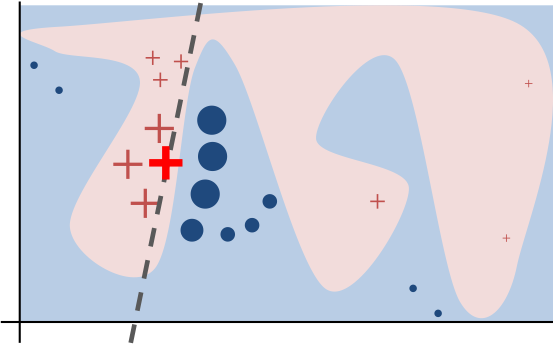
\includegraphics[width=0.5\columnwidth]{master_thesis/gfx/lime.png}
\caption{Toy example to present intuition for LIME. Figure from~\cite{ribeiro2016i}}
\label{fig:lime}
\end{figure}

~\\$G$ is expressed using a linear model: $g(z^\prime) = w_g g^\prime$, and $\pi_x(z) = exp(-D(x, z)^2/\sigma^2)$, so $L(f,g,\pi_x)=\sum_{z,z^\prime \in Z}\pi_x(z)(f(z) - g(z^\prime))^2$.
For this kind of linear model, when the model to be explained is very complicated, or when it is locally non-linear, it is not good to use a linear model to explain it. In addition, if the input itself cannot be broken into parts and uses missing or existing to affect the output, there is no way to use this method to explain.
\subsubsection{Anchor}
Anchor~\cite{ribeiro2018anchors} proposed in a paper by Reberio on AAAI in October 2018, a continuation of LIME. Anchors explains individual predictions of any black-box classification model by finding a decision rule that anchors the prediction sufficiently. Like its predecessor, the anchors approach deploys a perturbation-based strategy to generate local explanations for predictions of black-box machine learning models. However, instead of surrogate models used by LIME, the resulting explanations are expressed as easy-to-understand IF-THEN rules, called anchors. These rules are reusable since they are scoped: anchors include the notion of coverage, stating precisely to which other possibly unseen instances they apply. 
An anchor $A$ is formally defined as follows:
\begin{equation}
\begin{aligned}
\mathbb{E}_{\mathcal{D}_x(z|A)}[1_{f(x)=f(z)}]\geq\tau,A(x)=1
\end{aligned}
\label{eqn:eq2}
\end{equation}
where $A$ is a set of predicates, i.e., the resulting rule or anchor, $D_x (\cdot|A)$ indicates the distribution of neighbors of $x$, $0 \leq \tau \leq 1$ specifies a precision threshold. Given an instance $x$ to be explained, a rule or an anchor $A$ is to be found, such that it applies to $x$, while the same class as for $x$ gets predicted for a fraction of at least $\tau$ of $x$'s neighbors where the same $A$ is applicable. $A$ rule's precision results from evaluating neighbors or perturbations (following $D_x (z|A)$) using the provided machine learning model (denoted by the indicator function $1_{f(x) = f(z)}$).
\begin{figure}[H]
\centering
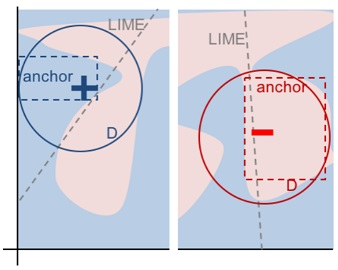
\includegraphics[width=0.5\columnwidth]{gfx/anchors-visualization.jpg}
\caption{LIME vs. Anchors. Figure from ~\cite{ribeiro2018anchors}}
\label{fig:Anchors}
\end{figure}

\subsubsection{Shapley Values}
Lundberg's 2017 approach to explain models through the SHAP\\ method~\cite{lundberg2017unified}. The main idea of the SHAP method is the shapley value. The Shapley value is a method derived from cooperative game theory. The Shapley value created by Shapley in 1953 is a method of allocating expenses to players based on their contribution to the total expenditure. Players cooperate in the alliance and get a certain benefit from this cooperation. If you use the value to explain the prediction of machine learning, "Total Expenditure" is the model prediction value of a single instance of the data set, "Player" is the characteristic value of the instance, and "Return" is the actual prediction of the instance minus the average of all instances prediction.
We are interested in how each feature affects the prediction. It is easy to calculate the contribution of each feature in a linear model. Here is what a linear model prediction looks like for one data instance:
\begin{equation}
\begin{aligned}
\hat{f}(x)=\beta_0+\beta_{1}x_{1}+\ldots+\beta_{p}x_{p}
\end{aligned}
\label{eqn:eq3}
\end{equation}
where $x$ is the instance for which we want to compute the contributions. Each $x_j$ is a feature value, with $j = 1,...,p$. The $\beta_j$ is the weight corresponding to feature $j$.
The contribution $\phi_j$ of the j-th feature on the prediction $\hat{f}(x)$ is:
\begin{equation}
\begin{aligned}
\phi_j(\hat{f})=\beta_{j}x_j-E(\beta_{j}X_{j})=\beta_{j}x_j-\beta_{j}E(X_{j})
\end{aligned}
\label{eqn:eq4}
\end{equation}
The shapley value of a feature value is its contribution to the payout, weighted and summed over all possible feature value combinations:
\begin{equation}
\begin{aligned}
\phi_j(val)=\sum_{S\subseteq\{x_{1},\ldots,x_{p}\}\setminus\{x_j\}}\frac{|S|!\left(p-|S|-1\right)!}{p!}\left(val\left(S\cup\{x_j\}\right)-val(S)\right)
\end{aligned}
\label{eqn:eq5}
\end{equation}
where $S$ is a subset of the features used in the model, $x$ is the vector of feature values of the instance to be explained and p the number of features. $val_x(S)$ is the prediction for feature values in set $S$.
First, select an instance of interest $x$, a feature $j$ and the number of iterations $M$. For each iteration, a random instance $z$ is selected from the data and a random order of the features is generated. Two new instances are created by combining values from the instance of interest $x$ and the sample $z$. The first instance $x_{+j}$ is the instance of interest, but all values in the order before and including value of feature $j$ are replaced by feature values from the sample $z$. The second instance $x_{-j}$ is similar,it has all the values in the order before, but excluding feature $j$ replaced by values of feature $j$ from the sample $z$. The difference in the prediction from the black box is computed:
\begin{equation}
\begin{aligned}
\phi_j^{m}=\hat{f}(x^m_{+j})-\hat{f}(x^m_{-j})
\end{aligned}
\label{eqn:eq6}
\end{equation}
All these differences are averaged and result in:
\begin{equation}
\begin{aligned}
\phi_j(x)=\frac{1}{M}\sum_{m=1}^M\phi_j^{m}
\end{aligned}
\label{eqn:eq7}
\end{equation}
Averaging implicitly weighs samples by the probability distribution of $X$. The procedure has to be repeated for each of the features to get all shapley values.

Like many other permutation-based interpretation methods, the shapley value method suffers from inclusion of unrealistic data instances when features are correlated. 

\subsection{Example-Based Methods}

\subsubsection{Adversarial}
The adversarial sample refers to the fact that when a small change is made to a certain feature value of a sample, the entire model makes a wrong prediction, this concept was proposed in Szegedy~\cite{szegedy2013intriguing}. The goal of adversarial samples is to deceive models, and the means by which hackers attack machine learning models is often to find these adversarial examples.
\begin{figure}[H]
\centering
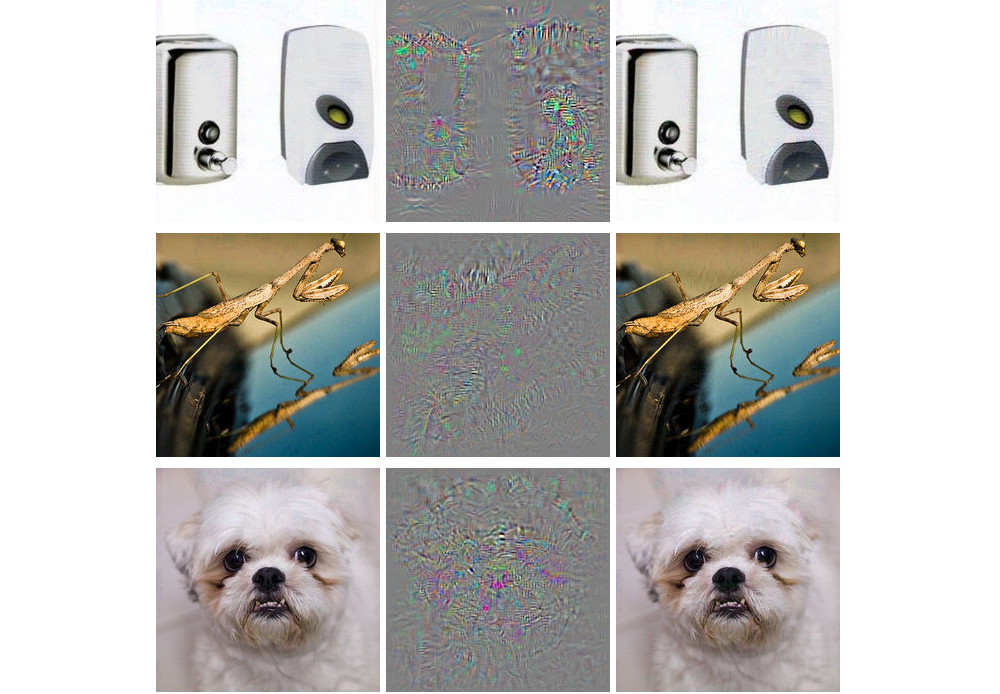
\includegraphics[width=0.5\columnwidth]{gfx/adversarial-ostrich.jpg}
\caption{Adversarial examples for AlexNet from ~\cite{szegedy2013intriguing}}
\label{fig:Adversarial}
\end{figure}
~\\These adversarial examples were generated by minimizing the following function:
\begin{equation}
\begin{aligned}
loss(\hat{f}(x+r),l)+c\cdot|r|
\end{aligned}
\label{eqn:eq8}
\end{equation}
~\\where x is an image, r is the changes, l is the desired outcome class, and the parameter c is used to balance the distance between images and the distance between predictions. 
\\\\Zhao~\cite{zhao2017generating} proposed a method to generate more natural, legible adversarial samples, which can be used to measure the robustness of the model. The steps are as follows:
\\\\1. Train a generator $G_{\theta}:Z\to X$ using WGAN~\cite{arjovsky2017wasserstein} and (unlabeled) real data X.
\\\\2. Train its inverse function $I_{\gamma}:X\to Z$ according to the generator.The specific training way is as follows:
\begin{equation}
\begin{aligned}
\underset{\gamma}{\mathrm{min}} \quad E_{x\sim p(x)}(\lVert G_\theta(I_\gamma(x)) - x\rVert) + \lambda\cdot E_{z\sim p(z)}(L(z,I_\gamma(G_\theta(z))))
\end{aligned}
\label{eqn:eq10}
\end{equation}
\\\\3. For a specific real data $x$, use $I_{\gamma}$ to map it back to the hidden space, that is, $z'=I_\gamma(x)$, and then randomly perturb $z'$ on the hidden space to get $\tilde{z}$, and finally $\tilde{x}=G_\theta(\tilde{z})$ gets the corresponding adversarial sample.
\\\\The adversarial samples generated based on this method will be more natural in appearance.

\subsubsection{Counterfactual}
The counterfactual explanation is like saying "If X didn't happen, Y wouldn't happen".
\begin{figure}[H]
\centering
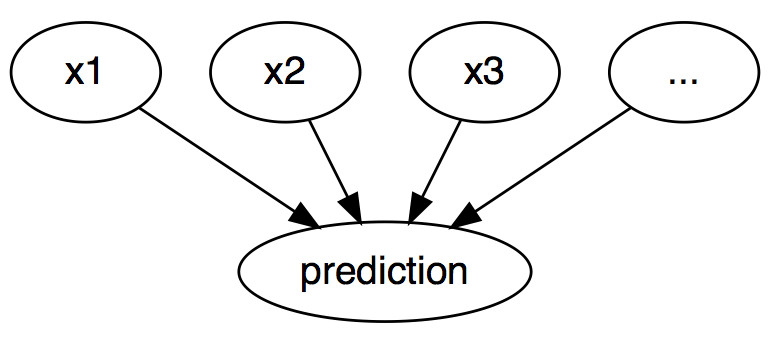
\includegraphics[width=0.5\columnwidth]{gfx/counterfactual.jpg}
\caption{The causal relationships between inputs of a machine learning model and the predictions.Figure from ~\cite{molnar2019}}
\label{fig:counterfactual}
\end{figure}
~\\We do this by changing a feature of a sample and then observing the change in the prediction result. Google's what if tool~\cite{wexler2019whatif} can help us do this analysis.


